% Yvonnick Esnault - yvonnick.e@free.fr 
% Gaetan Le Brun - gaetan.lebrun@gmail.com
% Thibaut Leli�vre - thibaut.lelievre@voila.fr
% Vincent Mah� - vmahe@free.fr
% Les chapitres peuvent commencer sur une page paire ou impaire
%openany
\documentclass[a4paper,11pt]{article}
%\frontmatter

\usepackage[T1]{fontenc}
\usepackage{ae,aecompl}
\usepackage[frenchb]{babel}
\usepackage[pdftex]{graphicx}
\usepackage[french]{minitoc}
\usepackage{fancyhdr}
\usepackage{lastpage}
\usepackage{hyperref}
\usepackage{textcomp}
%\usepackage [applemac] {inputenc} % les accents
\usepackage{verbatim}
\usepackage{float}

\evensidemargin=13pt
\oddsidemargin=13pt
\topmargin=-\headheight \advance\topmargin by -\headsep
\textwidth=14.59cm \textheight=21.62cm % normal A4, 1'' margin % 24.62cm
\setlength{\parindent}{8mm} % on remet le retrait de paragraphe

%%% My Vars %%%
\def\mytitle{TetraHead}
\def\mysubject{Synth\'etiseur}
\def\mydate{\today}
\def\myversion{1.0}
\def\me{\small  Yvonnick Esnault - Ga�tan Le Brun - Thibaut Leli�vre - Vincent Mah�}
\def\meandmail{\me \\{\normalsize\tt \mymail}}

%%% Fancy headers to add logo, line \ldots{} %%%
\pagestyle{fancy}
\fancyhf{}

% red�finition du style plain pour les pages sp�ciales (chapter)
\fancypagestyle{plain}{
 \fancyhead{}
 \renewcommand{\headrulewidth}{0pt}
 \renewcommand{\footrulewidth}{0.4pt}
 \lfoot{\textsl{\me\space} \\
\mysubject}
 \cfoot{}
 \rfoot{\textsl{Page \thepage \space sur \pageref{LastPage} }}
}

\renewcommand{\headsep}{50pt}

%\renewcommand{\chaptermark}[1]{\markboth{#1}{}}
\renewcommand{\sectionmark}[1]{\markright{#1}}
%\lhead[\thepage]{\rightmark}
%\rhead[\leftmark]{\thepage}

% Header
%\lhead{\includegraphics[width=2cm]{../document_type/images/logo.png}}
\chead{\mysubject} %\leftmark : contient le nom du chapitre courant.
%\rhead{\includegraphics[width=2cm]{images/logo_itin.png}}

%Footer
\lfoot{\textsl{\me\space}}
\cfoot{}
\rfoot{\textsl{Page \thepage \space sur \pageref{LastPage} }}

%Affiche les ligne en haut, et en bas
\renewcommand{\headrulewidth}{0.4pt}
\renewcommand{\footrulewidth}{0.4pt}

%%% bookmarks, linking in pdf %%%
\hypersetup{pdfauthor={\me},%
            pdftitle={\mytitle},%
            pdfsubject={\mysubject},%
            colorlinks,%
            citecolor=black,%
            filecolor=black,%
            linkcolor=black,%
            urlcolor=black,%
            pdftex}

%%% Commande pour supprimer en-t�tes
%%% et pied de page des pages vides
\newcommand{\clearemptydoublepage}{%
\newpage{\pagestyle{empty}\cleardoublepage}}

%%% Environnement pour le tableau de l'historique
\newenvironment{historique}
{

\begin{center}
{\huge \textbf{Historique}}

\vspace{3cm}
\begin{tabular}{|l|l|l|l|}
\hline
\textbf{Date} & \textbf{Auteur} & \textbf{Modifications} & \textbf{Version} \\
\hline
}
{
\end{tabular}\end{center}
\newpage
}

\newcommand{\histo}[4]
{#1 & #2 & #3 & #4 \\
\hline
}


%\newcommand{\info}[1]{
%\begin{figure}
%  \framebox[\textwidth][l]{
%   \begin{minipage}[c]{0.1\textwidth}
%     \medskip
%
%      
\includegraphics{../document_type/images/info.png}
%      \medskip
%
%   \end{minipage} \hfill
%   \begin{minipage}[c]{0.8\textwidth}
%     \medskip
%
%     #1\medskip
%
%   \end{minipage} \hfill
%   \begin{minipage}[c]{0.1\textwidth}
%     \makebox[30pt]{}\par
%   \end{minipage}
%}
%\end{figure}
%}

\newcommand{\encadre}[2]{
\begin{figure}[!h]
  \framebox[\textwidth][l]{
   \begin{minipage}[c]{0.1\textwidth}
     \medskip

      \includegraphics{#1}
      \medskip

   \end{minipage} \hfill
   \begin{minipage}[c]{0.8\textwidth}
     \medskip

     #2\medskip

   \end{minipage} \hfill
   \begin{minipage}[c]{0.1\textwidth}
     \makebox[30pt]{}\par
   \end{minipage}
}
\end{figure}
}

\newcommand{\info}[1]{
\encadre{../document_type/images/info.png}{#1}
}

\newcommand{\attention}[1]{
\encadre{../document_type/images/attention.png}{#1}
}

\newcommand{\code}[1]{\texttt{#1}}

\newcommand{\subsubsubsection}[1]{\textbf{#1}
\medskip

}

\usepackage{makeidx}
\usepackage{eepic}
\usepackage{xspace}

\newcommand{\tth}{\textsc{TetraHead}\xspace}

\newcommand{\titre}{Guide de l'utilisateur}
\newcommand{\diffusion}{\textbf{Libre} & Restreint & Confidentiel}
\newcommand{\etat}{Applicable}
\newcommand{\version}{1.0}
\newcommand{\datedoc}{15/02/06}

\makeindex

\begin{document}
%\pagenumbering{Arabic}

\newlength{\larg}
\setlength{\larg}{14.5cm}

\begin{titlepage}

\begin{center}

\includegraphics{../document_type/images/logo_TetraHead_small.png}\\
\end{center}
 
 %\vspace{5.5cm}
 \vspace{\stretch{1}}

{\rule{\larg}{1mm}}\vspace{7mm}
\begin{center}
  {\Huge {\bf {TetraHead - Synth\'etiseur}}} \\
  \medskip
  {\huge \titre}
\end{center}

\vspace{2mm}

{\rule{\larg}{1mm}}
\vspace{2mm} \\
\begin{tabular}{p{11cm} r}
   & {\large \bf 2006}% \\
%   & {\large  \today}
\end{tabular}\\
%\vspace{3cm}
\vspace{\stretch{1}}

\medskip

\begin{center}
\begin{tabular}{|l|l|l|l|}
\hline
\textbf{Diffusion} & \diffusion \\
\hline
�tat & \multicolumn{3}{|l|}{\textbf{\etat}} \\
\hline
Version & \multicolumn{3}{|l|}{\textbf{\version}} \\
\hline
Date & \multicolumn{3}{|l|}{\textbf{\datedoc}} \\
\hline
\end{tabular}

\end{center}

\end{titlepage}



\begin{historique}
\histo{09/02/2006}{Thibaut Leli�vre}{Cr�ation}{1.0}
\histo{10/02/2006}{Thibaut Leli�vre}{Tutorial}{1.1}
\histo{13/02/2006}{Yvonnick Esnault, Vincent Mah�}{Description des modules}{1.2}
\histo{13/02/2006}{Vincent Mah�}{Installation}{1.3}
\histo{14/02/2006}{Thibaut Leli�vre, Vincent Mah�}{Relecture}{1.4}
\end{historique}
\newpage

\tableofcontents
\newpage
\listoffigures
\newpage

\section{Pr�sentation}

Ce document est le manuel de l'utilisateur. Il explique comment se servir du 
logiciel \tth.

Dans ce document, on peut trouver des apart�s de deux types : des informations 
suppl�mentaires comme, par exemple, des trucs et astuces, et des avertissements.
Ces apart�s sont mis dans des encadr�s :

\info{Ceci est une information suppl�mentaire.}

\attention{Il faut faire attention � cette information.}




\section{Installation de \tth}
\label{installation}
\index{Installation}

\subsection{Configuration requise}
\begin{description}
\index{Processeur}
\item[Processeur :] CISC (Intel Pentium\texttrademark, AMD 
Athlon\texttrademark, \ldots) ou RISC (IBM PowerPC\texttrademark, Motorola 
Power G4/5\texttrademark, Sun UltraSparc\texttrademark, \ldots) cadenc� � 2 GHz 
ou plus.
\item[Syst�me d'exploitation :] tout syst�me r�cent pour lequel existe un 
environnement Java 5.0\texttrademark.
\item[Runtime :] \index{Java}Java Runtime Environment (JRE) 5.0\texttrademark
\item[Mat�riel :] carte son reconnue par le syst�me d'exploitation et g�r�e par 
Java 5.0.
\end{description} 

\subsection{Contr�les}

V�rification de la version de java install�e sur la machine

\subsubsection{sur MacOS X}
\index{Installation!MacOS}
\begin{verbatim}
	$ /System/Library/Frameworks/JavaVM.framework/Versions/1.5.0/Commands/java -version
	   java version "1.5.0_05"
	   Java(TM) 2 Runtime Environment, Standard Edition (build 1.5.0_05-83)
	   Java HotSpot(TM) Client VM (build 1.5.0_05-48, mixed mode, sharing)
	$ tar xjf tetrahead.tar.bz2
	$ cd tetrahead
\end{verbatim}

Commande de lancement de \tth � mettre en raccourci :\\
\begin{verbatim}
	$ /System/Library/Frameworks/JavaVM.framework/Versions/1.5.0/Commands/java -jar tetrahead.jar
\end{verbatim} 

\subsubsection{sur Linux}
\index{Installation!Linux}
\begin{verbatim}
	$ /usr/java/jdk1.5.0_03/bin/java -version
	   java version "1.5.0_03"
	   Java(TM) 2 Runtime Environment, Standard Edition (build 1.5.0_03-b07)
	   Java HotSpot(TM) Client VM (build 1.5.0_03-b07, mixed mode, sharing)
	$ tar xjf tetrahead.tar.bz2
	$ cd tetrahead
\end{verbatim} 

Commande de lancement de \tth � mettre en raccourci :
\begin{verbatim}
	$ /usr/java/jdk1.5.0\_03/bin/java -jar tetrahead.jar
\end{verbatim}

\subsubsection{sur Windows}
\index{Installation!Windows}
Ouvrir une console, faire :
\begin{verbatim}
	$ java -version
	   java version "1.5.0_06"
	   Java(TM) 2 Runtime Environment, Standard Edition (build 1.5.0_06-b05)
	   Java HotSpot(TM) Client VM (build 1.5.0_06-b05, mixed mode, sharing)
\end{verbatim} 

D�compresser le fichier \code{tetrahead.tar.bz2} dans le r�pertoire de votre choix.\\
Il s'y cr��e alors un sous-r�pertoire \code{tetrahead}.
\medskip

Pour mettre en raccourci la commande de lancement de \tth, faire un clic droit sur 
le fichier \code{tetrahead.jar}, puis choisir \emph{Cr�er un raccourci}.\\
Faire un double clic sur le raccourci ainsi cr�� pour lancer \tth.


\section{D�marrage}

\subsection{Commande}

\begin{enumerate}
\item Ouvrir une fen�tre de commande.
\item Passer dans le r�pertoire \code{tetrahead}.
\item Ex�cuter la commande \code{java -jar tetrahead.jar}
\end{enumerate}

\subsection{Probl�mes pouvant �tre rencontr�s}
\index{Problemes@Probl�mes}
\begin{description}
\item[Ne trouve pas l'ex�cutable :] passer le chemin complet de l'ex�cutable 
Java (cf. section~\ref{installation}, page~\pageref{installation}).

\item[Fichier tetrahead.jar corrompu :] t�l�charger � nouveau le logiciel \tth, 
puis le r�installer (cf. section~\ref{installation}, 
page~\pageref{installation}).

\end{description} 
\section{Conventions graphiques}

\subsection{Description de la fen�tre}

\begin{figure}[!htpb]
  \begin{center}
	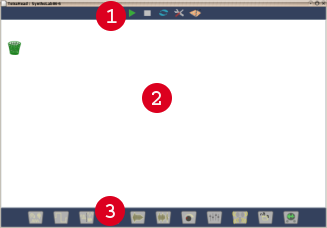
\includegraphics{images/screenshot}
    \caption{Capture d'�cran de la fen�tre principale}
  \end{center}
\end{figure}

Elle compte trois zones :
\begin{enumerate}
\item Une barre d'outils de commandes, \index{Barre d'outils!Commandes}situ�e 
en haut de la fen�tre
\item Un espace de travail\index{Espace de travail},
\item Une barre d'outils de cr�ation de modules\index{Barre d'outils!Creation 
de modules@Cr�ation de modules}, en bas de la fen�tre.
\end{enumerate}

\subsection{La barre d'outils de commande}

Avec cette barre d'outils, lancer (ou arr�ter) l'ex�cution du syntht�tiseur. 
Elle comporte cinq boutons :
\begin{itemize}
\item Un bouton \emph{Lecture} \index{Lecture}: Cliquer sur ce bouton pour 
d�marrer l'ex�cution du synth�tiseur.
\item Un bouton \emph{Arr�t} \index{Arret@Arr�t}: Cliquer sur ce bouton pour 
stopper l'ex�cution du synth�tiseur.
\item Un bouton \emph{Reset} \index{Reset}: Cliquer sur ce bouton pour remettre 
� $0$ tous les param�tres de tous les modules.
\item Un bouton \emph{Options} \index{Options}: Cliquer sur ce bouton pour changer les options du synth�tiseur, � savoir la fr�quence d'�chantillonnage utilis�e pour la version actuelle.
\item Un bouton \emph{A propos de...} \index{About}: Cliquer sur ce bouton pour en savoir plus sur les auteurs de \tth.
\end{itemize}

Lancer la lecture d�sactive les boutons \emph{Lecture} et \emph{Reset} et active le bouton 
\emph{Arr�t}. Arr�ter la lecture d�sactive le bouton \emph{Arr�t} et active les 
boutons \emph{Lecture}et \emph{Reset}.

\subsection{L'espace de travail}

Dans cette zone, cr�er les modules d�sir�s, les connecter, modifier leurs 
param�tres pour lancer ensuite l'ex�cution du synth�tiseur.

Si cette zone est trop petite pour voir tous les modules cr��s, des ascenseurs 
apparaissent pour faire d�filer la vue.

Cette zone contient une corbeille. D�poser un module au-dessus de cette 
corbeille \index{Corbeille}supprime ce module. Cette corbeille peut �tre d�plac�e.

\subsection{La barre d'outils de cr�ation de modules}

Avec cette barre d'outils\index{Barre d'outils!Creation 
de modules@Cr�ation de modules}, cr�er vos modules dans l'espace de travail en faisant 
glisser un bouton vers la zone de travail. Les boutons sont :

\begin{itemize}
\item VCO
\item LFO
\item VCF
\item VCF Param
\item ADHSR
\item ADSRTrigger
\item VCA
\item Mixer
\item OUTDirect
\item OUTFile
\item Oscilloscope
\end{itemize}

Chaque bouton cr�e un module du m�me nom. Pour plus d'informations sur ces 
modules, se reporter � la section~\ref{secDescModules}, 
page~\pageref{secDescModules}.

\subsection{Description d'un module}

Tous les modules \index{Module}sont dessin�s de la m�me fa�on.\\
Voici, par exemple, le module VCO :

\begin{figure}[!htpb]
  \begin{center}
    % screen shot d'un VCO
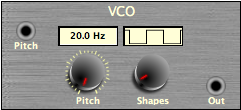
\includegraphics[scale=0.7]{images/module_vco.png}
    \caption{Capture d'�cran de la fen�tre principale}
  \end{center}
\end{figure}

Les modules \index{Module!Description}sont compos�s de la fa�on suivante : 
\bigskip

\begin{center}
	\begin{tabular}{|c|c|c|}
	\hline \multicolumn{3}{|c|}{Nom du module} \\ 
	\hline ports & param�tres continus  & port de \\ 
				   d'entr�e & et discrets & sortie \\ 
				   &  & \\ 
	\hline
	\end{tabular} 
\end{center}
\bigskip

Chaque module poss�de un nombre quelconque de ports d'entr�es, un nombre 
quelconque de param�tres et au plus un port de sortie.

Les param�tres sont des boutons que l'on peut tourner avec la souris. Il existe 
deux types de param�tres : les param�tres discrets et continus. � l'�cran, un 
param�tre continu est entour� de graduations, contrairement � un param�tre 
discret.

\subsubsection{Les param�tres discrets}
\index{Parametre@Param�tre!Discret}
Un param�tre discret se modifie en cliquant sur le bouton. Un clic droit tourne 
le bouton d'un cran vers la droite, tandis qu'un clic gauche le ram�ne vers la 
gauche.

Les param�tres discrets ne peuvent prendre qu'une certaine valeur parmi une 
liste finie de valeurs. Par exemple, pour le VCO, le param�tre \emph{Shapes} 
(le param�tre � droite) ne peut prendre comme valeurs que \emph{Carr�}, 
\emph{Toit d'usine}, \emph{Dents de scie}, \emph{Triangle}, ou \emph{Sinuso�de}, 
repr�sent�s.par une image correspondante de l'onde.

\subsubsection{Les param�tres continus}
\index{Parametre@Param�tre!Continu}
La valeur d'un param�tre continu appartient � un certain intervalle. Par 
exemple, pour le VCO, le param�tre \emph{Pitch} (� gauche) prend une valeur 
entre 20 Hz et 3520 Hz.

Pour tourner le bouton, il faut appuyer dessus avec le bouton de la souris puis 
la d�placer autour du centre. La valeur augmente quand on tourne le bouton vers 
la droite.

Avec la souris, il est difficile d'obtenir une valeur pr�cise. Aussi \tth 
permet de saisir exactement la valeur d�sir�e au clavier dans la zone de texte 
juste au dessus du bouton.

\section{Premiers pas}

Cette partie du manuel explique comment cr�er un premier montage avec
quelques modules.

\subsection*{\'Etape 1}

D�marrer \tth pour afficher l'�cran principal.

\subsection*{\'Etape 2 : Cr�ation de modules}

Dans la barre d'outils en bas de l'�cran, se trouvent les boutons de cr�ation 
de modules. Cliquer (mais sans relacher le bouton de la souris) sur un bouton 
\emph{VCO} de la barre d'outils inf�rieure :
\begin{center}
	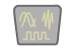
\includegraphics{tutorial/vco.png}
\end{center}

Puis d�placer la souris dans l'espace de travail. Un module est apparu � 
l'�cran. Il peut �tre d�plac� n'importe o� dans l'espace de travail.

Recommencer l'op�ration avec un module \emph{OUTDirect} :
\begin{center}
	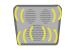
\includegraphics{tutorial/out.png}
\end{center}

Pour savoir quels sont les r�les de ces modules, se reporter � la 
section~\ref{secDescModules}, page~\pageref{secDescModules}.
L'�cran doit ressembler � ceci :
\begin{center}
	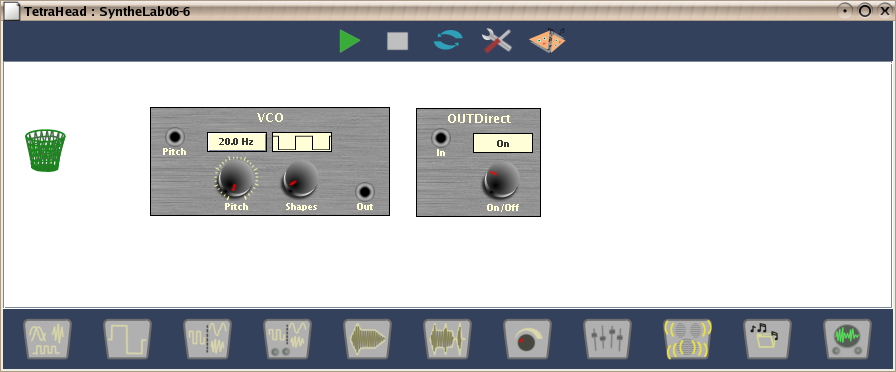
\includegraphics[width=\textwidth]{tutorial/etape2.png}
\end{center}

\subsection*{\'Etape 3 : Connexion de modules}

Pour g�n�rer du son, il faut connecter ces deux modules ensemble en r�alisant 
un glisser-d�placer avec la souris depuis un port de sortie vers un port 
d'entr�e.
\begin{center}
	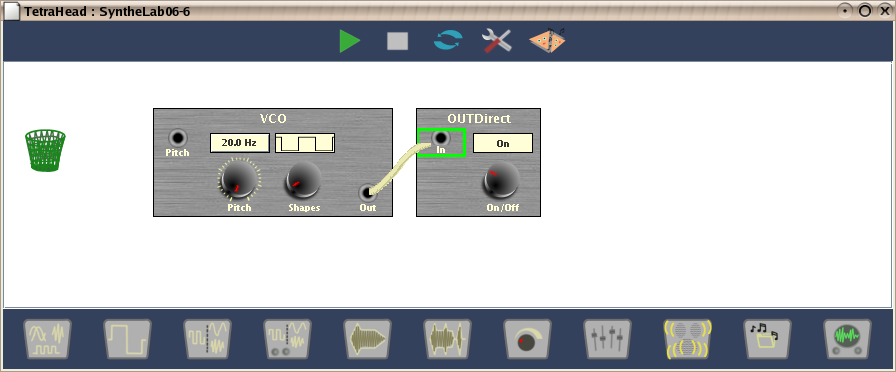
\includegraphics[width=\textwidth]{tutorial/etape3.png}
\end{center}

\info{Pendant le glisser-d�placer, une bordure verte appara�t autour du port 
d'entr�e pour indiquer que la connexion est autoris�e. Si le port d'entr�e 
�tait d�j� connect�, la connexion aurait �t� refus�e et la bordure serait rouge.
}

\subsection*{�tape 4 : Modification d'un param�tre discret}

Le VCO compte deux param�tres : un discret, � droite, et un continu � gauche. 
Cliquer 4 fois avec le bouton droit de la souris sur le bouton \emph{Shapes}
du VCO. Cela fait tourner le bouton du param�tre d'un cran vers la droite � 
chaque clic droit (r�ciproquement avec un clic gauche). La courbe repr�sent�e 
doit normalement �tre une sinuso�de :
\begin{center}
	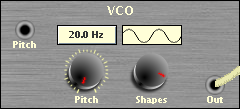
\includegraphics[scale=0.7]{tutorial/etape4.png}
\end{center}

\subsection*{�tape 5 : Modification d'un param�tre continu}

Cliquer (sans relacher) sur le bouton \emph{Pitch} du VCO. Cela modifie la 
valeur du param�tre, valeur que l'on peut voir dans l'�tiquette au-dessus du 
bouton.

Tourner le bouton jusqu'� obtenir une fr�quence de $440Hz$. Avec la souris, il 
est difficile d'obtenir un r�sultat aussi pr�cis. Pour y rem�dier, il faut 
utiliser le clavier. S�lectionner tout le contenu de l'�tiquette :

Saisir \emph{440} au clavier, puis taper \emph{Entr�e} :
\begin{center}
	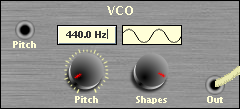
\includegraphics[scale=0.7]{tutorial/etape5-2.png}
\end{center}

\subsection*{�tape 6 : Synth�se du son}

Ce montage est un montage minimum pour produire du son. Cliquer sur le bouton 
de lecture (triangle vert dans la barre d'outils en haut de la fen�tre) pour 
commencer la synth�se du son. Le bouton rouge est le bouton d'arr�t.

Avec ce montage, le son produit est un La comme on peut l'obtenir avec un 
diapason ou en d�crochant son t�l�phone.

\subsection*{�tape 7 : Suppression d'un fil}

Arr�ter la synth�se du son. Cliquer avec le bouton droit de la souris sur le fil
connectant les deux modules pour le supprimer.

\attention{Il n'est possible ni de supprimer un fil, ni d'ajouter ou supprimer des 
modules pendant la synth�se de son.}

\subsection*{�tape 8 : Suppression d'un module}

Pour supprimer un module, il suffit de le jeter dans la corbeille � papiers pr�sente sur l'espace de travail.

\info{La corbeille, comme les modules, est d�pla�able dans l'espace de travail. 
On peut donc la placer o� l'on veut.}




\newpage
\section{Description des modules}
\label{secDescModules}

\subsection{Oscillateurs}

\subsubsection{VCO}

\begin{figure}[!h]
 \begin{center}
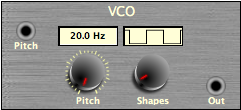
\includegraphics[height=2cm]{images/module_vco.png}
 \caption{Le module VCO}
 \end{center}
\end{figure}

Le VCO (\textbf{V}oltage \textbf{C}ontrolled \textbf{O}scillator) permet de 
g�n�rer un signal, c'est l'�l�ment de base dans un montage. Il est constitu� de 
deux boutons, respectivement de gauche � droite : Pitch et Forme d'onde. Le 
Picth permet de r�gler la fr�quence de l'onde g�n�r�e. Par exemple, pour avoir 
la note LA de base, il suffit de mettre la valeur � 440 Hz.

Le second bouton permet de modifier la forme d'onde g�n�r�e qui peut �tre de la forme : 

\begin{description}
\item [Onde Carr�e :] 
\includegraphics[width=2cm]{images/Square.png}

\item [Onde Sinuso�dale :] 
\includegraphics[width=2cm]{images/Sine.png}

\item [Onde Dents de scie :] 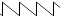
\includegraphics[width=2cm]{images/Saw_tooth.png}

\item [Onde Factory Roof :] 
\includegraphics[width=2cm]{images/Factory_roof.png}

\item [Onde Triangulaire :] 
\includegraphics[width=2cm]{images/Triangle.png}

\end{description}

Le VCO poss�de �galement un port d'entr�e, nomm� Pitch-IN. Suivant la valeur 
du signal re�u, il permet d'ajouter ou de supprimer des harmoniques au signal 
g�n�r�. C'est g�n�ralement un LFO qui est banch� � ce port.

\subsubsection{LFO}

\begin{figure}[!h]
 \begin{center}
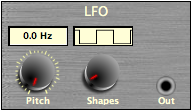
\includegraphics[height=2cm]{images/module_lfo.png}
 \caption{Le module LFO}
 \end{center}
\end{figure}

Le LFO (\textbf{L}ow \textbf{F}requency \textbf{O}scillator) permet de g�n�rer 
un signal � base fr�quence. Il est constitu� de deux boutons, respectivement de 
gauche � droite : Pitch et Forme d'onde. Le Picth permet de r�gler la fr�quence 
de l'onde g�n�r�e, de 0 � 20 Hz. G�n�ralement, le LFO est r�gl� � une fr�quence 
tr�s basse (entre 0.1 et quelques Hz).

Le second bouton permet de modifier la forme d'onde g�n�r�e, voir la 
documentation sur le VCO � ce sujet. %\newpage

\subsection{Enveloppes}

\info{L'ADHSR et l'ADSR Trigger d�crits ci-dessous ne pas des g�n�rateurs 
d'enveloppe proprement dit. Ils poss�dent tous les deux un port d'entr�e, c'est 
sur le signal re�u sur ce port d'entr�e qu'une enveloppe va �tre produite en 
sortie.}

\subsubsection{ADHSR}

\begin{figure}[!h]
 \begin{center}
 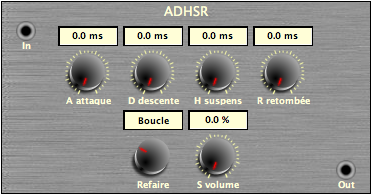
\includegraphics[height=2cm]{images/module_adhsr.png}
 \caption{Le module ADHSR}
 \end{center}
\end{figure}

ADHSR : \textbf{A}ttack, \textbf{D}ecay, \textbf{H}old, \textbf{S}ustain, 
\textbf{R}elease.

\subsubsection{ADSR Trigger}

\begin{figure}[!h]
 \begin{center}
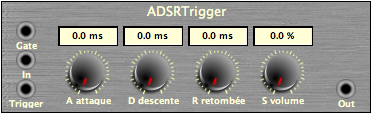
\includegraphics[height=2cm]{images/module_adsrtrigger.png}
 \caption{Le module ADSR Trigger}
 \end{center}
\end{figure}

L'ADSR Trigger poss�de plusieurs comportements suivant les valeurs qu'il re�oit
sur ces ports d'entr�e \code{gate} et \code{trigger}.  

\begin{figure}[!h]
 \begin{center}
 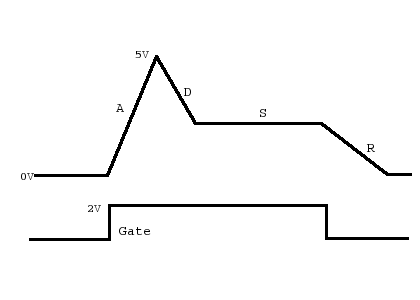
\includegraphics[height=5cm]{images/ADSR_1.png}
 \caption{Enveloppe classique : une gate sans trigger.}
 \end{center}
\end{figure}


\begin{figure}[!h]
 \begin{center}
 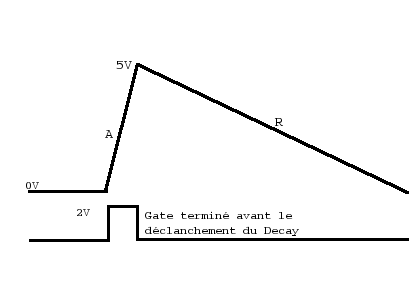
\includegraphics[height=5cm]{images/ADSR_2.png}
 \caption{La gate se termine avant le d�clenchement du Decay, le Release se d�clenche.}
 \end{center}
\end{figure}


\begin{figure}[!h]
 \begin{center}
 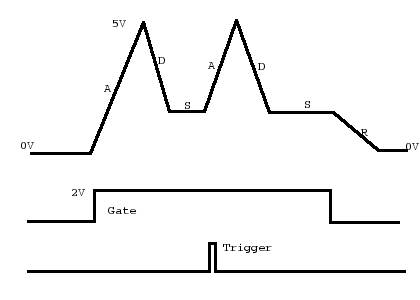
\includegraphics[height=5cm]{images/ADSR_3.png}
 \caption{Utilisation d'un trigger au milieu d'une gate : g�n�ration d'une nouvelle attaque}
 \end{center}
\end{figure}


\begin{figure}[!h]
 \begin{center}
 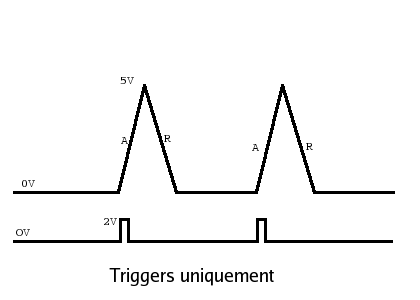
\includegraphics[height=5cm]{images/ADSR_4.png}
 \caption{Utilisation de triggers sans gate : aucun Decay n'est produit.}
 \end{center}
\end{figure}


\newpage
\subsection{Filtres}

\subsubsection{VCF}

\begin{figure}[!h]
 \begin{center}
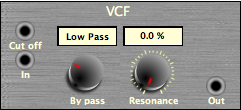
\includegraphics[height=2cm]{images/module_vcf.png}
 \caption{Le VCF}
 \end{center}
\end{figure}

Le VCF (\textbf{V}oltage \textbf{C}ontrolled \textbf{F}ilter) permet 
d'appliquer soit un filtre \emph{Passe-Haut}, soit un filtre 
\emph{Passe-Bas} sur le signal re�u sur le port d'entr�e.

En compl�ment du port d'entr�e IN, ce module poss�de un second port d'entr�e : 
\emph{Cut-off In}. Le signal re�u sur cette entr�e permet de donner la 
fr�quence de coupure du filtre. Lorsque l'entr�e \emph{Cut-Off In} et le 
bouton \emph{Cut Off} sont positionn�s, c'est la moyenne des deux qui est 
appliqu�e en tant que fr�quence de coupure.

Le bouton \emph{R�sonnance} permet d'ajouter un effet d'�cho au signal filtr�.

\subsubsection{Mixer}

\begin{figure}[!h]
 \begin{center}
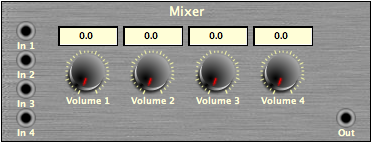
\includegraphics[height=2cm]{images/module_mixer.png}
 \caption{Le mixer}
 \end{center}
\end{figure}

Le mixer permet de m�langer plusieurs signaux, avec pour chaque signal la 
possibilit� de r�gler son volume. Il n'est pas obligatoire de brancher tous les 
ports d'entr�e du mixer.

\info{Un mixer branch� avec un seul port d'entr�e, r�gl� avec un volume entre 0 
et 100, � la m�me comportement qu'un VCA avec un gain r�gl� avec la m�me valeur 
que le volume.}

\subsubsection{VCA}

\begin{figure}[!h]
 \begin{center}
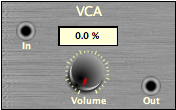
\includegraphics[height=2cm]{images/module_vca.png}
 \caption{Le module VCA}
 \end{center}
\end{figure}

Le VCA (\textbf{V}oltage \textbf{C}ontrolled \textbf{A}mplifier) permet 
d'amplifier un signal le signal re�u sur le port d'entr�e. Il est g�n�ralement 
utilis� � l'entr�e ou � la sortie d'un filtre.

\subsection{Sorties}

\subsubsection{OUT Direct}

\begin{figure}[!h]
 \begin{center}
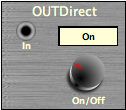
\includegraphics[height=2cm]{images/module_outdirect.png}
 \caption{Le module OUTDirect}
 \end{center}
\end{figure}

Le module OUT Direct poss�de un bouton ainsi qu'un port d'entr�e. Il permet de 
faire sortir sur les enceintes de l'ordinateur le signal re�u sur son port 
d'entr�e. Il faut s'assurer que le bouton soit positionn� sur l'�tat ON pour 
entendre le son.

\attention{ Remarque : il n'est pas possible d'avoir deux modules OUT Direct � l'�tat ON, 
lorsque le synth�tiseur est en cours de jeu.}

\subsubsection{OUTFile}

\begin{figure}[!h]
 \begin{center}
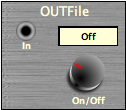
\includegraphics[height=2cm]{images/module_outfile.png}
 \caption{Le module OUTFile}
 \end{center}
\end{figure}

Le module OUT File permet de g�n�rer un fichier au format .wav. Le contenu de 
ce fichier correspond au signal qu'il re�oit sur son port d'entr�e.

Par d�faut, le fichier g�n�r� est plac� dans le r�pertoire \code{sorties/} et 
poss�de un nom tel que : sortie\_yyyymmdd\_hhmmssSS.wav o� y est l'ann�e, m le 
mois, d le jour, h l'heure etc \ldots

\subsubsection{Oscilloscope}

\begin{figure}[!h]
 \begin{center}
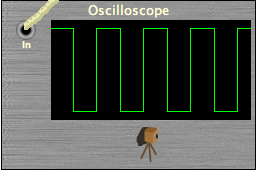
\includegraphics[height=2cm]{images/module_oscilloscope.png}
 \caption{Le module Oscilloscope}
 \end{center}
\end{figure}

L'oscilloscope permet de visualiser le signal re�u sur le port d'entr�e. 
L'ic�ne situ�e en dessous du graphique permet de stopper le d�filement du 
signal, ce qui est tr�s utile lorsque la fr�quence du signal est tr�s �lev�e. 
Un nouveau clic sur l'ic�ne fait repartir l'affichage.

\attention{Il n'est pas recommand� de faire fonctionner plus de trois 
oscillateurs sur un m�me montage. Ce module est gourmand en ressource 
processeur lorsqu'il n'est pas en pause.} \newpage

\section{Exemples de montages}
\label{exemples}

\subsection{Sonnerie d'un t�l�phone occup�}

\begin{figure}[!htpb]
	\begin{center} 
		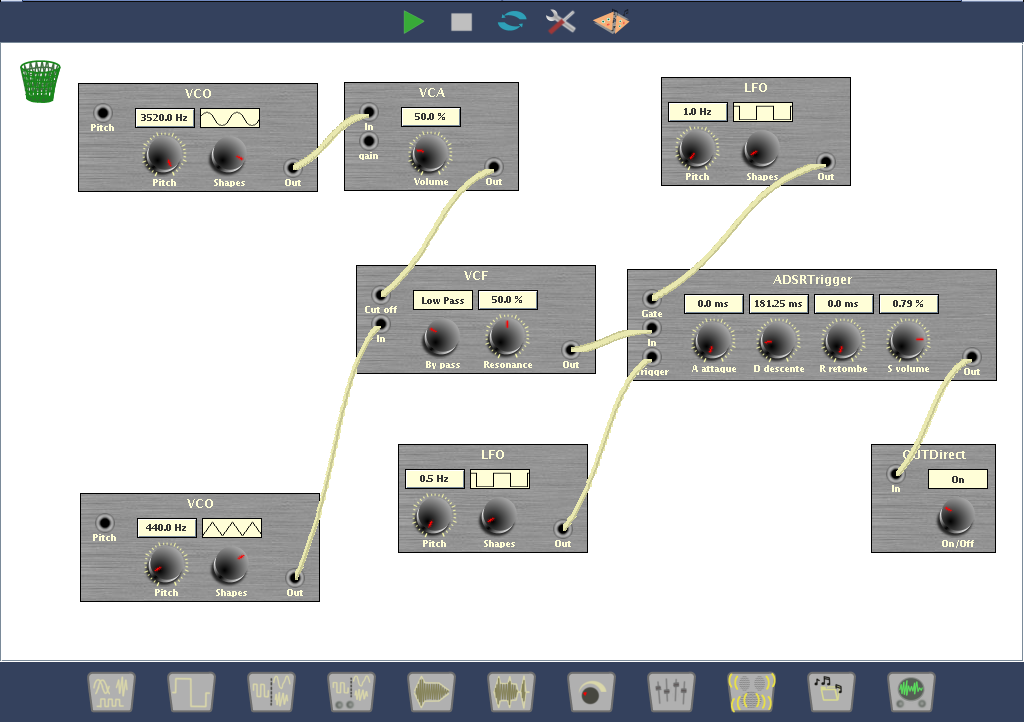
\includegraphics[width=\textwidth]{exemples/telephone_occupe.png}
		\caption{Montage pour faire une sonnerie de t�l�phone occup�}
	\end{center}
\end{figure}

\newpage

\subsection{Sir�ne de pompiers}

\begin{figure}[!htpb]
	\begin{center} 
		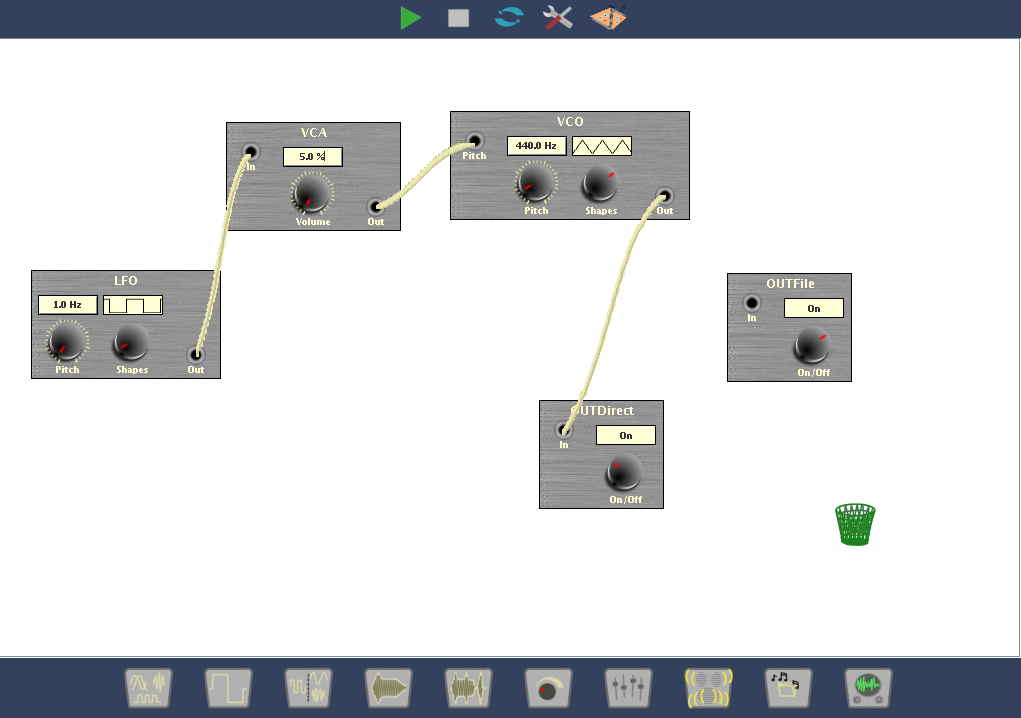
\includegraphics[width=\textwidth]{exemples/pompier.png}
		\caption{Montage pour faire une sir�ne de pompiers}
	\end{center}
\end{figure}

\newpage

\subsection{Sir�ne de policiers}

\begin{figure}[!htpb]
	\begin{center} 
		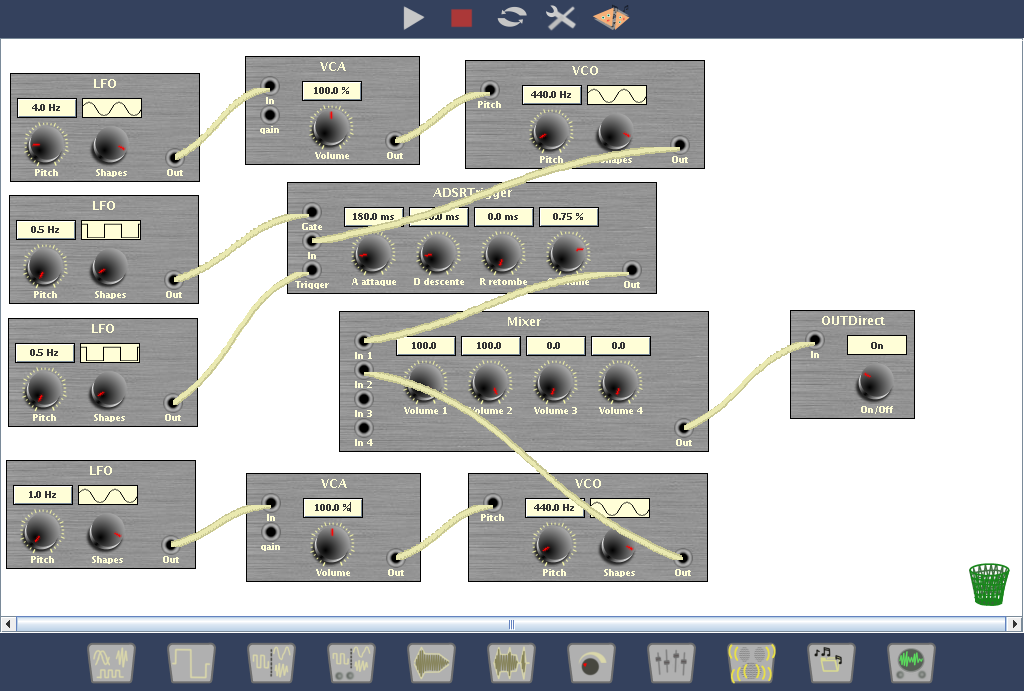
\includegraphics[width=\textwidth]{exemples/us_cops.png}
		\caption{Montage pour faire une sir�ne de policiers}
	\end{center}
\end{figure}




%\section{Glossaire}

\newpage

\printindex

\end{document}
